\documentclass[10pt, a4paper, twoside]{article}
\usepackage[utf8]{inputenc}
\usepackage{authblk}
\usepackage{multicol}
\usepackage{abstract}
\usepackage{xcolor}
\usepackage[a4paper, total={6in, 8in}]{geometry}
\usepackage{biblatex}
\usepackage{graphicx}
\usepackage{newfloat}
\DeclareFloatingEnvironment[name={Supplementary Figure},fileext=lsf,listname={List of Supplementary Figures}]{suppfigure}


\setlength{\columnsep}{1cm}
\addbibresource{su2020_cov2.bib}

\graphicspath{{../Figures/}}


\title{Impact of travel-associated cases on the SARS-CoV-2 epidemic in Switzerland from June to September 2020}

\author[1]{Martina L. Reichmuth}
\author[1]{Emma B. Hodcroft}
\author[1]{Julien Riou}
\author[2,3]{Niel Hens}
\author[1*]{Christian L. Althaus}

\renewcommand*{\Affilfont}{\normalsize\normalfont}
\affil[1]{Institute of Social and Preventive Medicine, University of Bern, Bern, Switzerland}
\affil[2]{Interuniversity Institute for Biostatistics and statistical Bioinformatics, Data Science Institute, Hasselt University, Hasselt, Belgium}
\affil[3]{Centre for Health Economics Research and Modelling Infectious Diseases, Vaccine and Infectious Disease Institute, University of Antwerp, Antwerp, Belgium}
\affil[*]{Correspondence: christian.althaus@ispm.unibe.ch}

\renewcommand{\abstractnamefont}{\normalfont\bfseries}
\renewcommand{\abstracttextfont}{\normalfont\small} 


\date{}
\pagenumbering{arabic}
\begin{document}
\maketitle
\begin{abstract}
\noindent 

Introduction: In Switzerland, the severe acute respiratory syndrome coronavirus 2 (SARS-CoV-2) epidemic grew from a few dozen confirmed cases to several hundred cases per day during summer 2020. 
Switzerland and other European countries opened borders to allow for holiday travel. 
The impact of travel-associated cases (imports) on the national epidemic dynamics remains unclear. 
Our objective was to assess the impact of imports on the epidemic from June to September 2020.

Method: We used the numbers of confirmed SARS-CoV-2 cases as reported by the Federal Office of Public Health (FOPH). 
We fitted a negative binomial generalised linear model to the daily number of confirmed cases to estimate the epidemic growth rate. 
We then used a stochastic branching process model that can account for individual variation in transmission of SARS-CoV-2 to simulate epidemic trajectories using different values for the effective reproduction number $R_e$ (0.6-1.2) and number of imports (3,304-14,582).

Results: From June to September 2020, 23,199 SARS-CoV-2 cases were reported. For 12,259 (52,84\%) cases the likely place of infection was reported, i.e. for 8,955 a national and 3,304 an international infection places were stated. 
In absence of imports, we estimated an epidemic growth rate of 0.023 (95\% confidence interval (CI): 0.021-0.024) per day. 
We found that increasing the number of imports requires lower values of $R_e$ to account for dynamic. 
For example, 3,304 imports (as reported) would have been sufficient to account for the observed epidemic dynamics despite $R_e$ < 1, i.e., a value below the critical threshold.

Discussion: Quantifying the role of imports on the national dynamics of SARS-CoV-2 epidemics requires further investigation. 
In Switzerland, imported cases might have had a considerable impact on the national dynamics and can explain the growth of the SARS-CoV-2 epidemic during summer 2020. 
Our results underline the importance of improved surveillance for international travellers in order to better control the spread of SARS-CoV-2.
\clearpage
\end{abstract}

\begin{multicols}{2}
\section{Introduction}
In spring 2020, travel-associated cases of the severe acute respiratory syndrome coronavirus 2 (SARS-CoV-2) were likely to have accounted for a high proportion of cases in many countries.\cite{russell_effect_2021} 
In the absence of travel restrictions, countries can expect travel-associated cases.\cite{russell_effect_2021} 
Thus, restrictions might contribute to epidemic control in many countries, whereas in others, travel-associated cases are likely to contribute little to local SARS-CoV-2 epidemics.\cite{russell_effect_2021}  
Russell et al., 2021 recommended that authorities evaluate the effect of travel-associated cases on the local SARS-CoV-2 incidence, local epidemic growth, and travel volumes before implementing such restrictions.\cite{russell_effect_2021} 
During summer 2020, Switzerland and other European countries had reopened borders to allow for travel. In Switzerland borders were reopened on the $15^{th}$ of June 2020 to \textcolor{red}{most/all (European)} countries. 
Due to Switzerlands prominent location in the heart of Europe - with boarders to Germany, France, Italy, Austria, and Principality of Liechtenstein - , many different countries are easily visited vis-versa many citizens from different countries might visit Switzerland. 
In summer 2020, Switzerland had a population of 8,5 millions and the SARS-CoV-2 epidemic grew from a few dozen confirmed cases per day in early June 2020 to several hundred cases per day by the end of September 2020. 

The dynamic of an epidemic can be explained with the effective reproduction number $R_e$. 
$R_e$ is the average number of secondary cases per infectious case in the population of both susceptible and non-susceptible individuals. 
If $R_e > 1$ , the number of cases will increase, where $R_e = 1$, the disease is endemic, and where $R_e < 1$ there will be a decline in the number of cases. 
For airborne disease such as SARS-CoV-2 the individual variation in transmission is difficult to measure empirically. 
Lloyd-Smith et al., 2005 showed that the population dynamic can be explained with mathematical models that allow for individual variation.\cite{lloyd-smith_superspreading_2005}  
Thus, secondary cases might be described with a negative binomial distribution. Depending on the over-dispersion parameter $k$ the probability of stochastic extinction and outbreaks varies widely. 
Disease control interventions could influence the individual variation in infectiousness.\cite{lloyd-smith_superspreading_2005} 
Lloyd-Smith et al., 2005 showed that outbreaks are rarer but more explosive and extinction is more likely with a small $k$ then with $k = 1$ equals the geometric distribution and $k = \infty$ that equals the Poisson distribution.\cite{lloyd-smith_superspreading_2005} 
Later accounts for no individual variation. 
Thus, the extinction probability in a stochastic model varies with $R_e$, $k$ and the number of infections at the start i.e. seeds. 
The $R_e$ can be estimated by the epidemic growth rate, the generation time resulting in a shape parameter, and rate parameter of the gamma distribution. 
The generation time is an interval when a susceptible is infected by an infected individual and when this individual was infected. These periods of infecting others can be explained using a gamma distribution. 
For SARS-CoV-2, the generation time was estimated to be 5.2 days with a standard deviation (SD) of 2.8.\cite{ganyani_estimating_2020}

The impact of travel-associated cases (in the method and result section called imports) on the Swiss national epidemic dynamics remains unclear. 
Our objective was to assess the impact of imports on the SARS-CoV-2 epidemic in Switzerland during summer 2020.

\section{Method}

\subsection{Data availability}
We analysed the epidemic from $1^{st}$ of June to $30^{th}$ of September 2020. 
For the propose of this study, we used confidential data reported by the Federal Office of Public Health (FOPH). 
Data included date of diagnosis, or registration, date of hospitalisation, and date of death. 
Moreover, most likely country of infection might be listed \textcolor{red}{so far not but would be interesting to use also age}.

\subsection{Definition}
$R_e$ is given by $(1 + \frac{r}{\beta} )^\alpha$ where $r$ is the epidemic growth rate, $\alpha$ the gamma shape parameter, and $\beta$ is the rate parameter of the gamma distribution. 
The parameter $\alpha$ is given by the generation time $\mu$ (here 5.2 days) and its variance $\sigma^2$ (here 7.8 days) as following $\frac{\mu^2}{\sigma^2 }$ and $\beta$ is given as following $\frac{\mu}{\sigma^2}$. 
The distribution of secondary cases can be descriped with a negative binomial distribution with the mean $R_e$ and the variance of $R_e$ as $\frac{R_e}{1+\frac{R_e}{k}}$ where $k$ is the over-dispersion parameter. 
The extinction probability in a stochastic model with a $k = \infty$ is given by $ P_{ext} = \frac{1}{R_e^n}$ where $n$ is the number of infections at the start i.e. seeds.\textcolor{red}{how for other k's?}

\subsection{Statistics}
We fitted a negative binomial generalised linear model to the daily number of confirmed cases, hospitalised cases, and deaths adjusted for weekends (using the MASS-package).\cite{venables_modern_2002} 
Later, we used these three models and estimated a weighted epidemic growth rate $r$ and the $R_e$ (as described in section 2.2). 
We predicted the epidemic curve for the time of interest ($1^{st}$ of June to $30^{th}$ of September 2020) with a seed of 50 cases on the $31^{st}$ of may. 
Further, we used a stochastic branching process model that can also account for individual variation in transmission of SARS-CoV-2 using an over-dispersion parameters $k$ of 0.1, 0.5, 1, and  $\infty$ to simulate epidemic trajectories. 
We included seeds for previous five days, i.e. 27$^{th}$  to 31$^{st}$ May 2020.
These seeds were estimated with the negative binomial generalised linear model on the daily number of confirmed cases multiplied with two. 
Further, we varied the $R_e$ (0.6-1.2 in 0.1 steps) value and number of imports in the stochastic branching model. 
We simulate epidemic trajectories including imports that transmitted further. 
We used reported imports, reported imports multiplied by following $1+ \frac{\Sigma ~of ~cases ~with ~unknown ~origin }{\Sigma ~of ~all ~confirmed ~cases}$. 
The number of imports per day were multiplied with 1, 2, and 3. As a sensitivity analysis, we allowed no further transmission for imports. 
All analyses were preformed using $R ~v.1.3.1093$.\cite{r_core_team_r_2020}


\subsection{Ethics}
\textcolor{red}{As we use FPOH data, do we have to state sth?}

\section{Results}
In total 23,199 cases were reported by the FOPH. For 12,259 (52,84\%) cases the likely place of infection was reported, i.e. for 8,955 a national and 3,304 an international infection places were stated. 
In absence of imports, we estimated an epidemic growth rate of 0.023 (95\%-confidence interval (CI): 0.021-0.024) per day and a $R_e$ of 1.044 95\%-CI: 1.041-1.047) for the time of interest. 
We found that increasing the number of imports requires lower values of $R_e$ to account for the observed dynamic in summer 2020 (Supplementary Figure 1). 
For example, 3,304 imports (as reported) would have been sufficient to account for the observed epidemic growth rate despite a national dynamic with $R_e$ 0.9, i.e., a value below the critical threshold of one (Figure 1). 
By extrapolating the imports regarding unknown origins of reported cases, already a $R_e$ 0.7 could explain the observed dynamic (Supplementary Figure 1b). 
Contrary, if imports did not further transmit a $R_e$ of 1.1-1.2 \textcolor{red}{higher than estimated R of 1.04?}would explain the observed dynamic (Figure1; Figure 2; Supplementary Figure 2). 
Whereas with imports that transmit further e.g. 3,304 and 4,862, an $R_e$ of 0.9-1.1 can partly explain the predicted case numbers per day (Figure 2). 
A increasing dispersion parameter (from 0.1 to $\infty$) narrowed the range of potential epidemics. Narrowing was also the increasing number of imported cases that transmit further (Figure 2; Supplementary Figure 3).
More extreme, wit 14,582 imports an $R_e$ of 0.8-0.9 can partly explain the predicted case numbers per day (Supplementary Figure 3). 
A smaller dispersion parameters allowed for a broader range of estimated growth rates (Figure 1). 
In general, reported or more imports that do not or do transmit further, account for a positive epidemic growth rate (Supplementary Figure 1; Supplementary Figure 2).
\textcolor{red}{In general I am a bit confused with the R values.. Figure1 vs Figure 2..}

\end{multicols}
\begin{figure}[h]
\centering
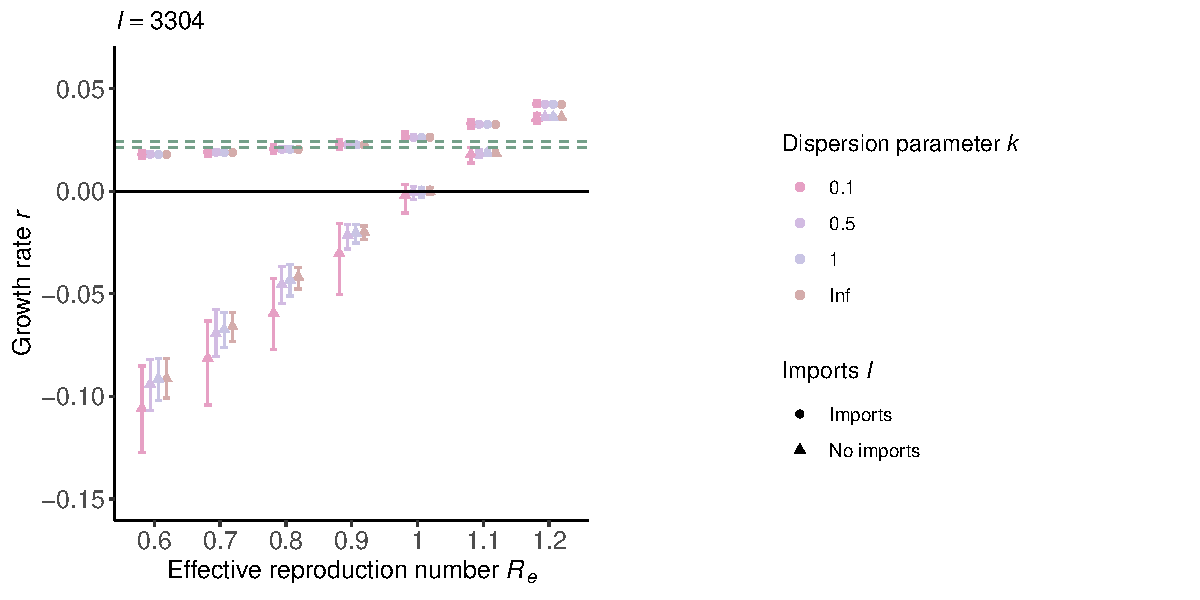
\includegraphics[scale=0.5]{growth_r_imports_infect_reported_2021-02-24.pdf}
\caption{Impact of imports on the epidemic growth rates: y-axis shows the epidemic growth rate; x-axis different $R_e$ values; intervals show the inter-quantile range (IQR). Abbreviations: k, dispersion parameter; I, number of imports.}
\end{figure}
\begin{multicols}{2}

\end{multicols}
\begin{figure}[h]
\centering
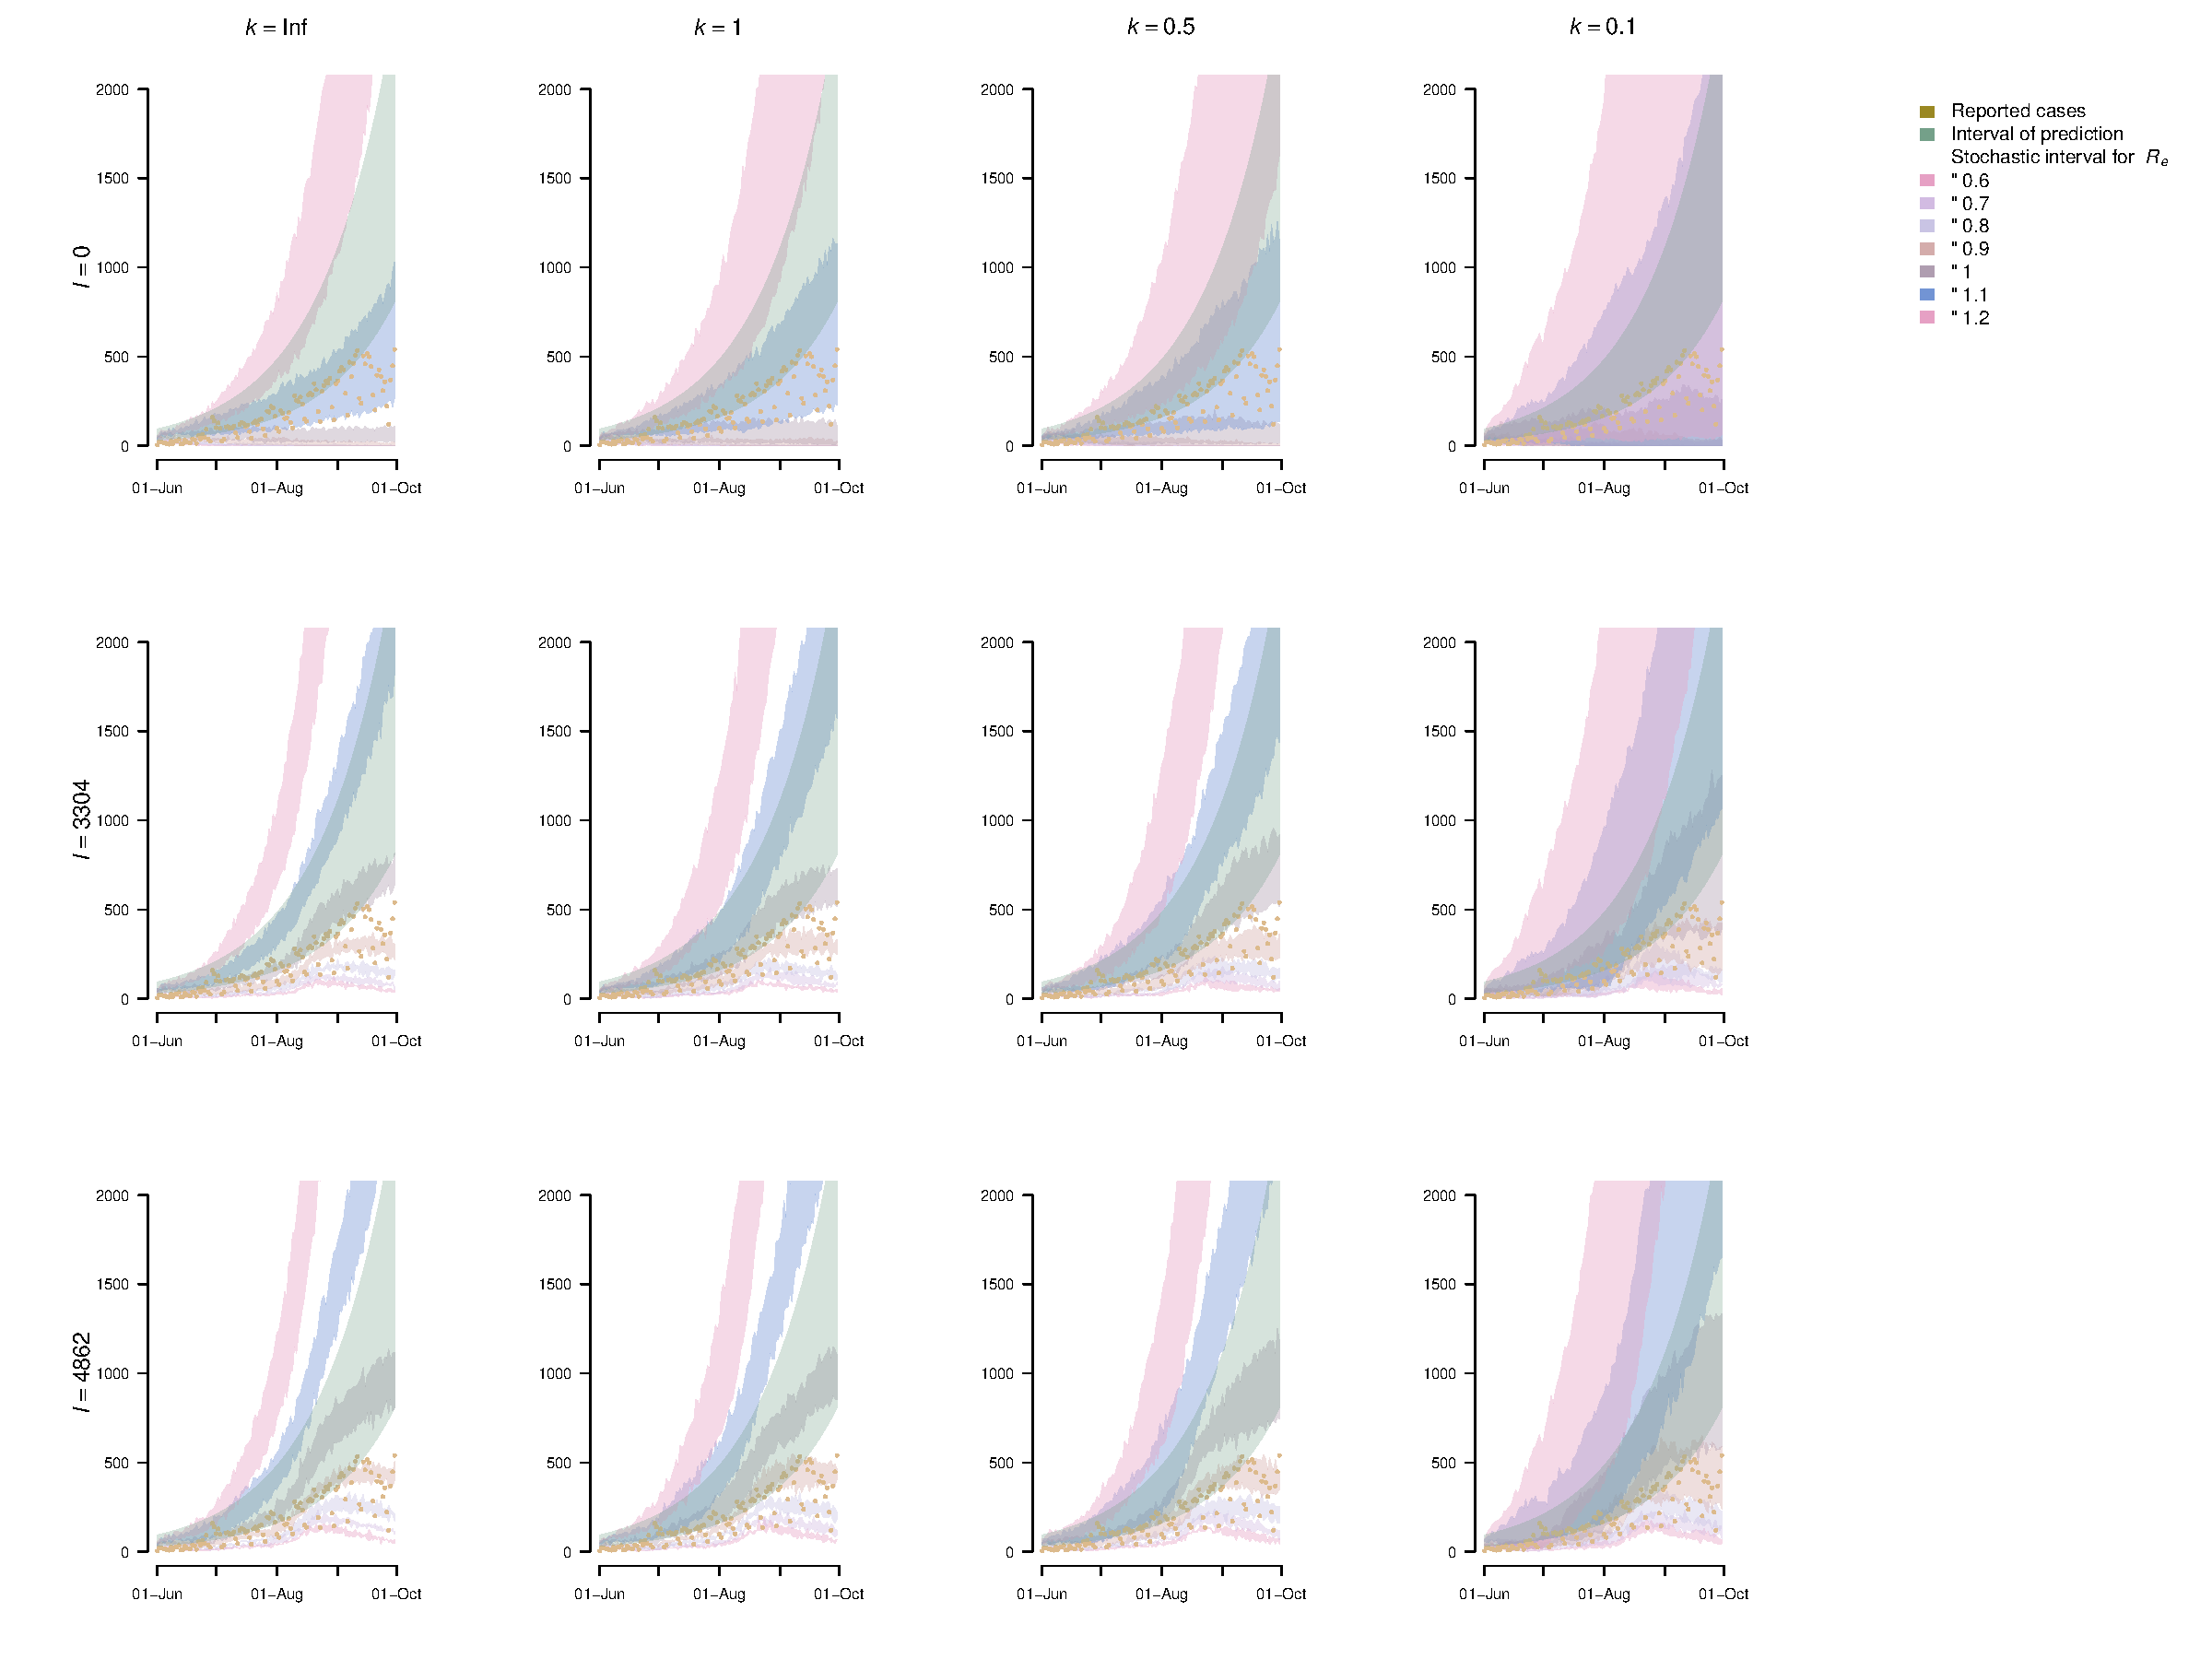
\includegraphics[scale=0.4]{sim3_cases_d_imports_infect_2021-02-24.pdf}
\caption{Impact of imports on the cases per day: y-axis shows the cases per day; x-axis the time of interest. Yellow dots show the reported cases per day and green area shows the predicted cases per day. Abbreviations: $k$, dispersion parameter; $I$, number of imports.}
\end{figure}

\begin{multicols}{2}

\section{Discussion}
The SARS-CoV-2 epidemic grew from a few dozen confirmed cases per day in early June 2020 to several hundred by the end of September 2020. 
Switzerland is a relative small country with a few millions citizens but due to is location (and prosperity) it has high potential that travel has a huge impact on the epidemic. 
Thus, the intrinsic large probability of extinction - due to small number of cases beginning of June - was potentially annulled by travel. 
We estimated a $R_e$ slightly above 1 for the time of interest. So, the $R_e$ value was around the critical value of 1, where small changes might have a huge effect on the epidemic. 
We showed that the national epidemic had a $R_e$ below one, i.e., a value below the critical threshold. 
Travel-associated cases and their further transmission consequently led to several hundred cases per day by the end of September 2020. 
Without any travel-associated cases, regardless of the dispersion parameter $k$, only an $R_e$ between 1.1 and 1.2 could explain the observed Swiss epidemic. 
In our analysis we only accounted that travel-associated case where successfully detected and thus stoped the transmission chain or that travel-associated case infected further in the same way as cases that were infected nationally.

\textcolor{red}{Nevertheless, our method has limitations that need to be addressed.}

Quantifying the role of imports on the national dynamics of SARS-CoV-2 epidemics requires further investigation. 
In Switzerland, travel-associated case might have had a considerable impact on the national dynamics and can explain the growth of the SARS-CoV-2 epidemic during summer 2020. 
Our results underline the importance of improved surveillance for international travellers in order to better control the spread of SARS-CoV-2.

\section{Acknowledgement}
We thank the FOPH.

\section{Author contributions}
MLR, EBH, JR, and CLR conceived the study and contributed to the analysis of the results. MLR performed the analysis and wrote the first draft of the manuscript. NH gave important inputs for the analysis and interpretation. All authors read and approved the final manuscript.

\section{Funding}
European Union’s Horizon 2020 research and innovation programme - project EpiPose (No 101003688). Swiss National Science Foundation (grant 196046)

\section{Reference}
\printbibliography[heading=none]

\end{multicols}

\clearpage
\section{Supplementary}
\begin{suppfigure}[h]
\centering
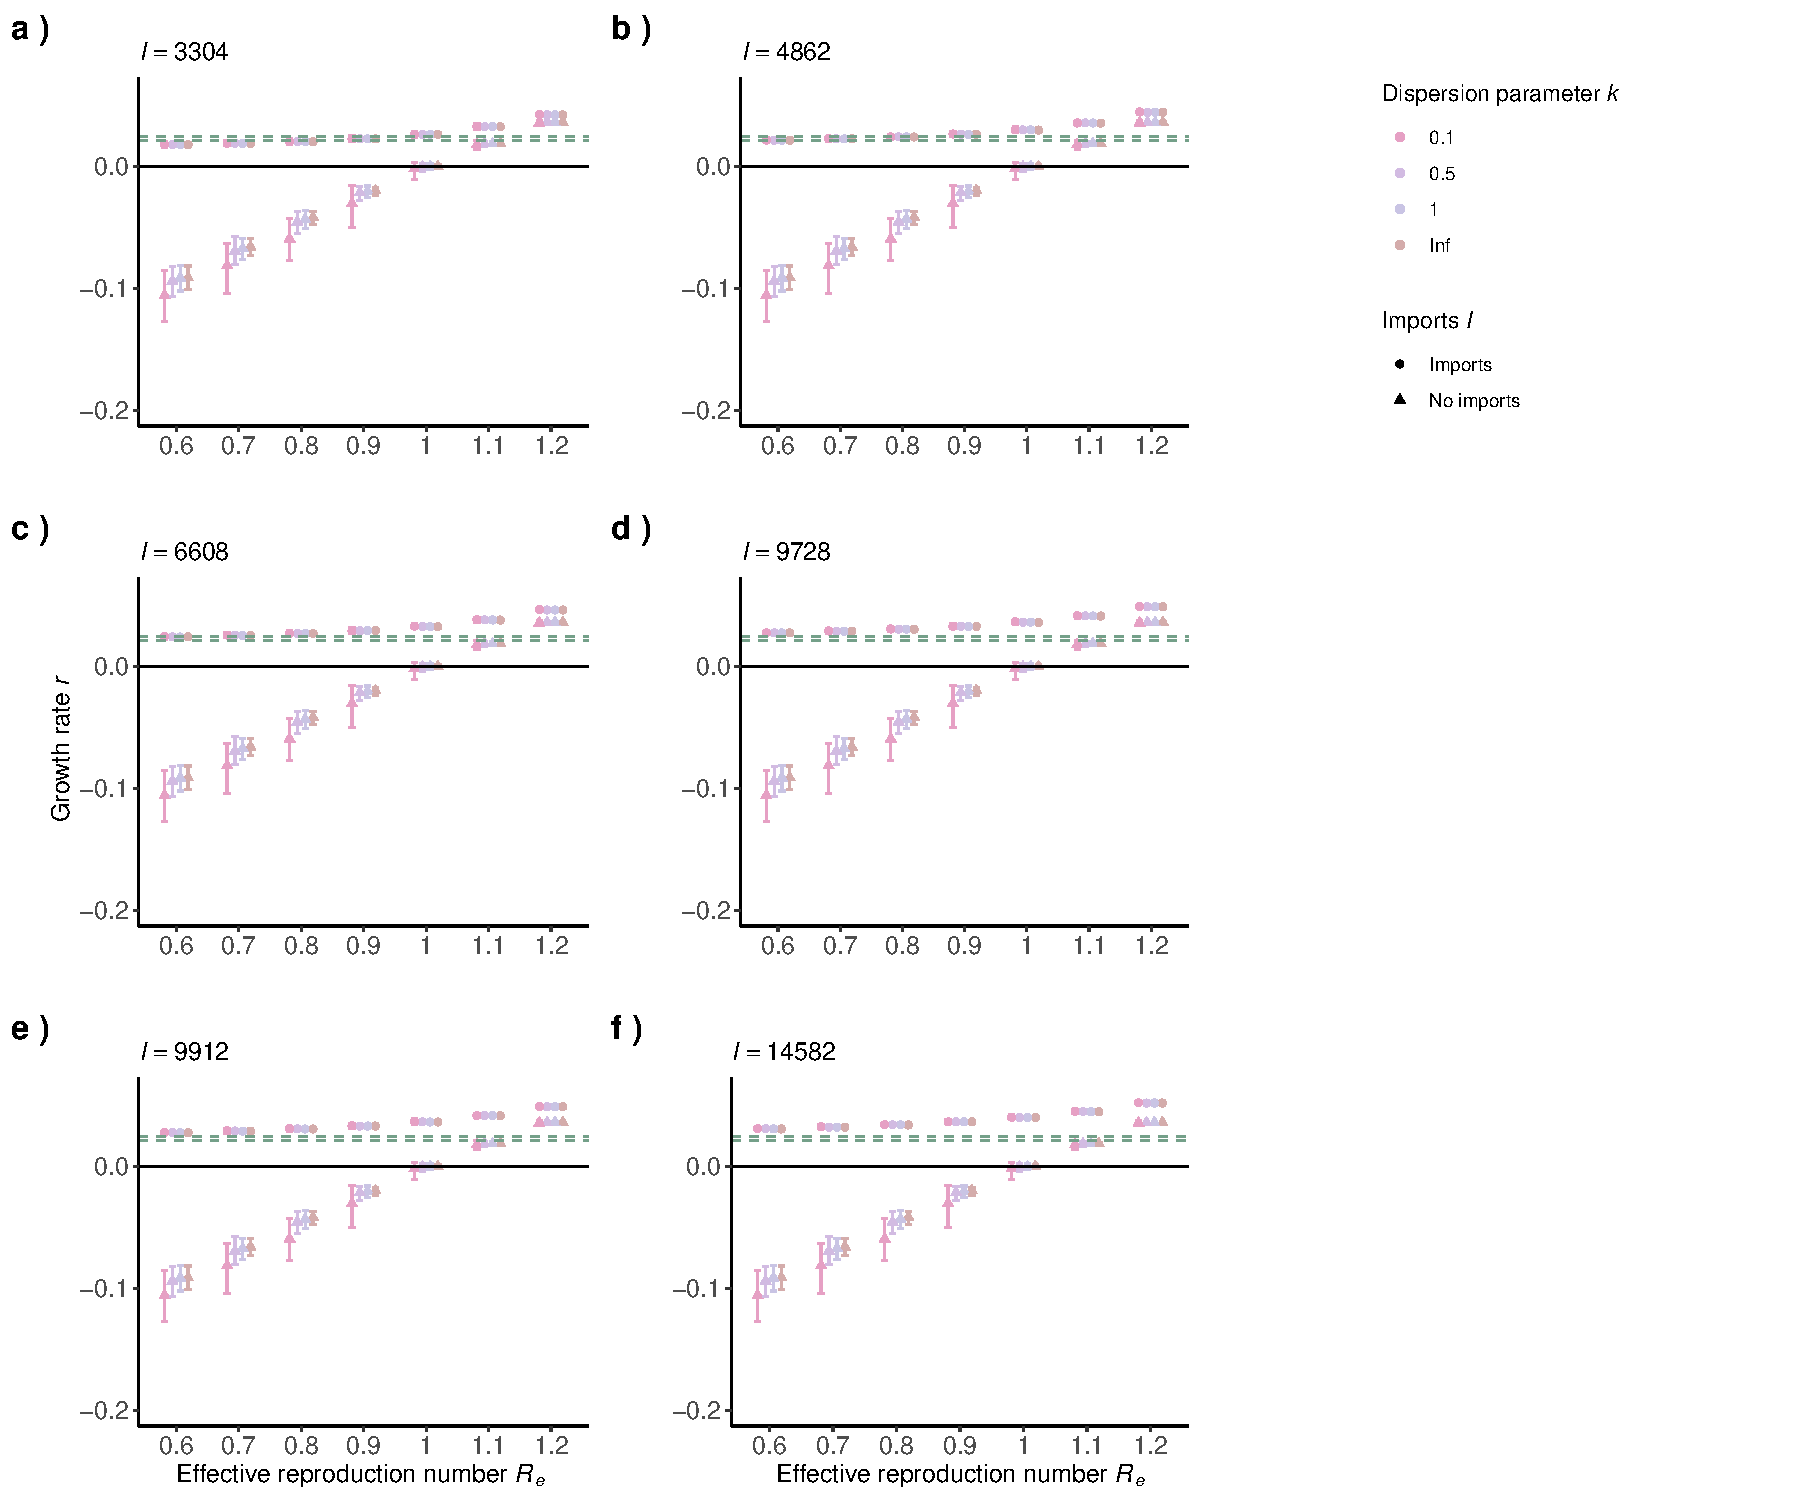
\includegraphics[scale=0.5]{growth_r_imports_infect_2021-02-24.pdf}
\caption{Impact of travel associated cases \emph{I} that infect further on the epidemic growth rates: y-axis shows the epidemic growth rate; x-axis different $R_e$ values; intervals show the inter-quantile range (IQR). a) reported travel associated cases. b) reported imports multiplied by following $1+ \frac{\Sigma ~of ~cases ~with ~unknown ~origin }{\Sigma ~of ~all ~confirmed ~cases}$. c) $a)$ multiplied with 2. d) $b)$ multiplied with 2. e,f) $a)$ and $b)$ multiplied with 3, respectively. Abbreviations: k, dispersion parameter; I, number of travel associated cases.}
\end{suppfigure}
\clearpage
\begin{suppfigure}[h]
\centering
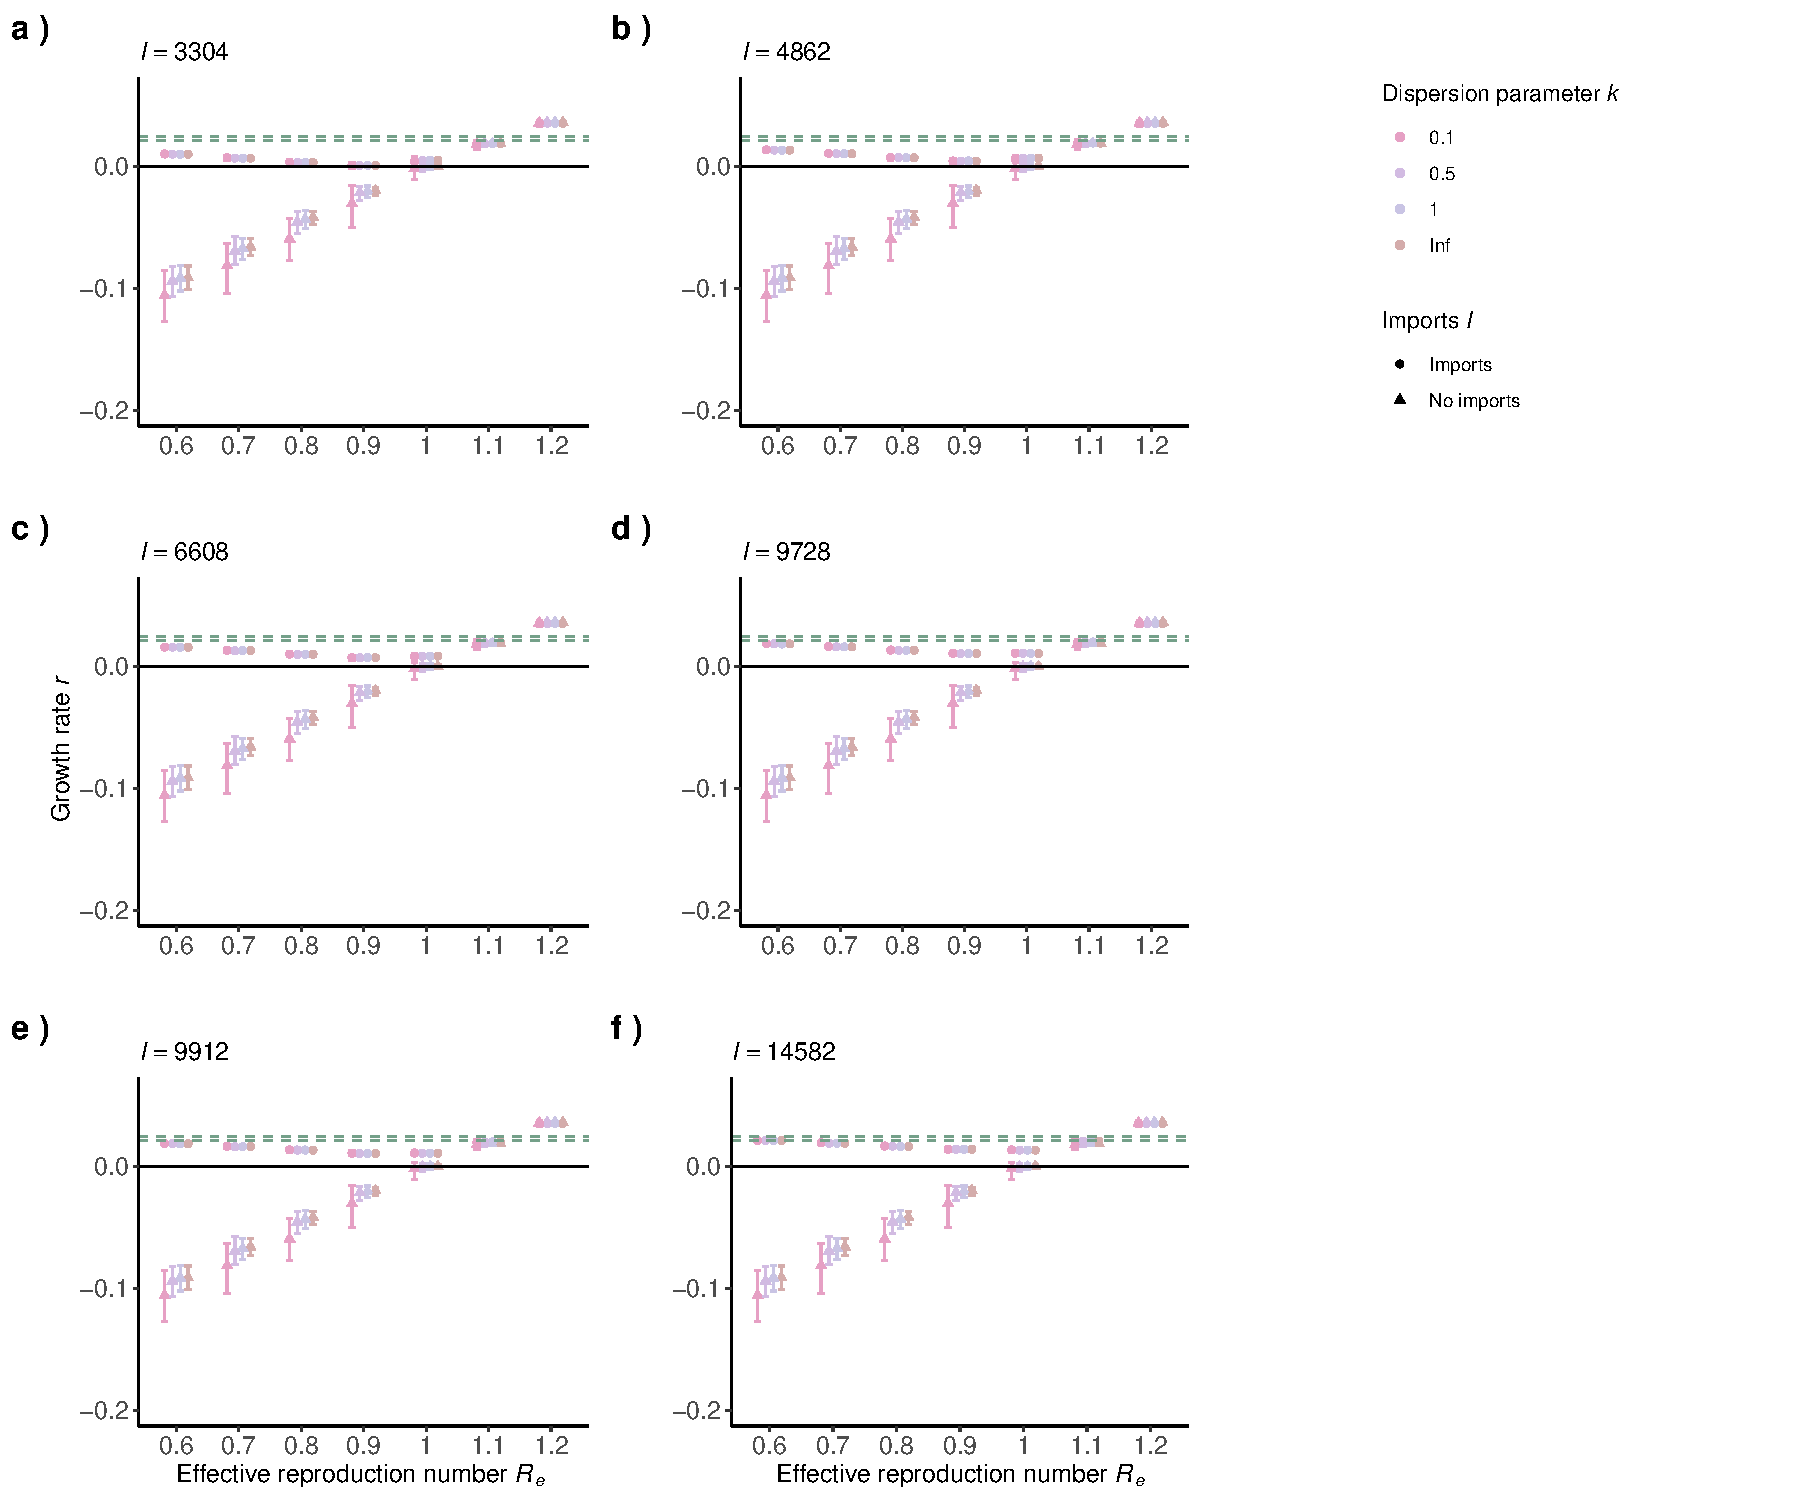
\includegraphics[scale=0.5]{growth_r_imports_2021-02-24.pdf}
\caption{Impact of travel associated cases \emph{I} that do not infect further on the epidemic growth rates: y-axis shows the epidemic growth rate; x-axis different $R_e$ values; intervals show the inter-quantile range (IQR). a) reported travel associated cases. b) reported imports multiplied by following $1+ \frac{\Sigma ~of ~cases ~with ~unknown ~origin }{\Sigma ~of ~all ~confirmed ~cases}$. c) $a)$ multiplied with 2. d) $b)$ multiplied with 2. e,f) $a)$ and $b)$ multiplied with 3, respectively. Abbreviations: k, dispersion parameter; I, number of travel associated cases.}
\end{suppfigure}
\begin{suppfigure}[h]
\centering
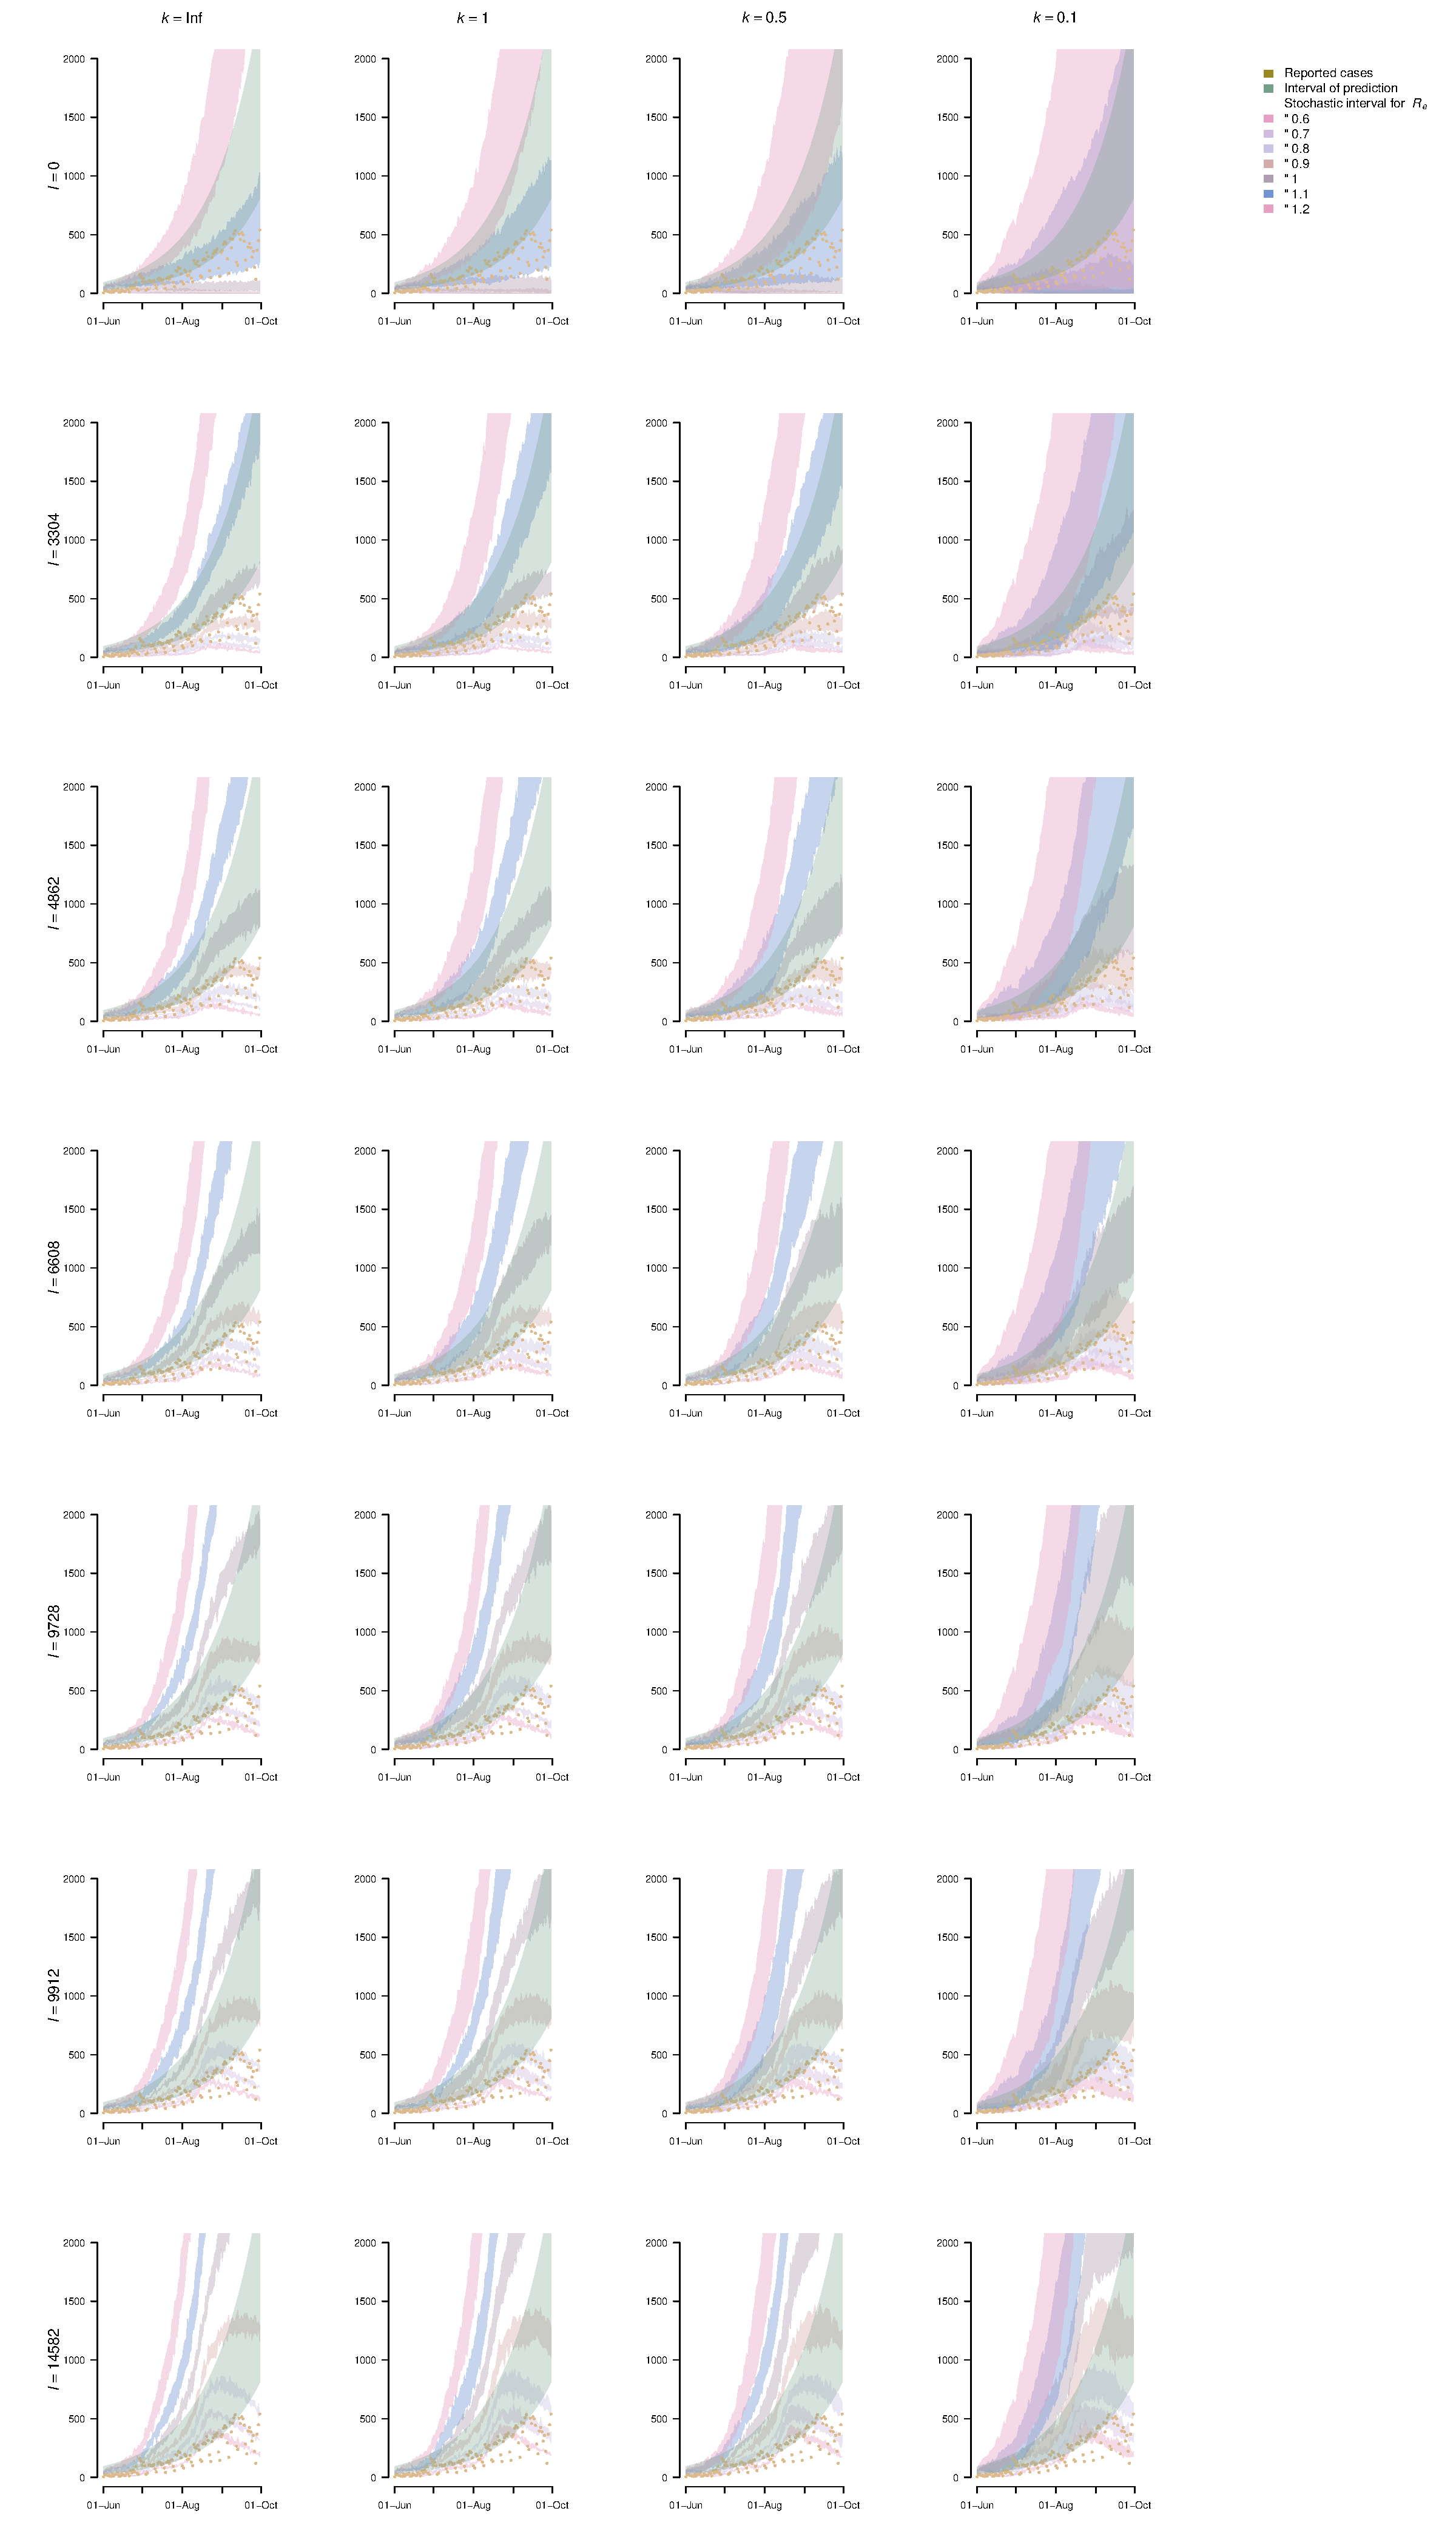
\includegraphics[scale=0.3]{sim_cases_d_imports_infect_2021-02-24.pdf}
\caption{Impact of travel associated cases on the cases per day that infect further: y-axis shows the cases per day; x-axis the time of interest. Different number of travel associated cases \emph{I} were added to a stochastic branching model whereby these \emph{I} could transmit further: \emph{I} was zero, reported \emph{I}, reported \emph{I} multiplied by $1+ \frac{\Sigma ~of ~cases ~with ~unknown ~origin }{\Sigma ~of ~all ~confirmed ~cases}$, and these multiplied with 2 and 3, respectively. Yellow dots show the reported cases per day and green area shows the predicted cases per day. Abbreviations: k, dispersion parameter; I, number of travel associated cases.}
\end{suppfigure}
\begin{suppfigure}[h]
\centering
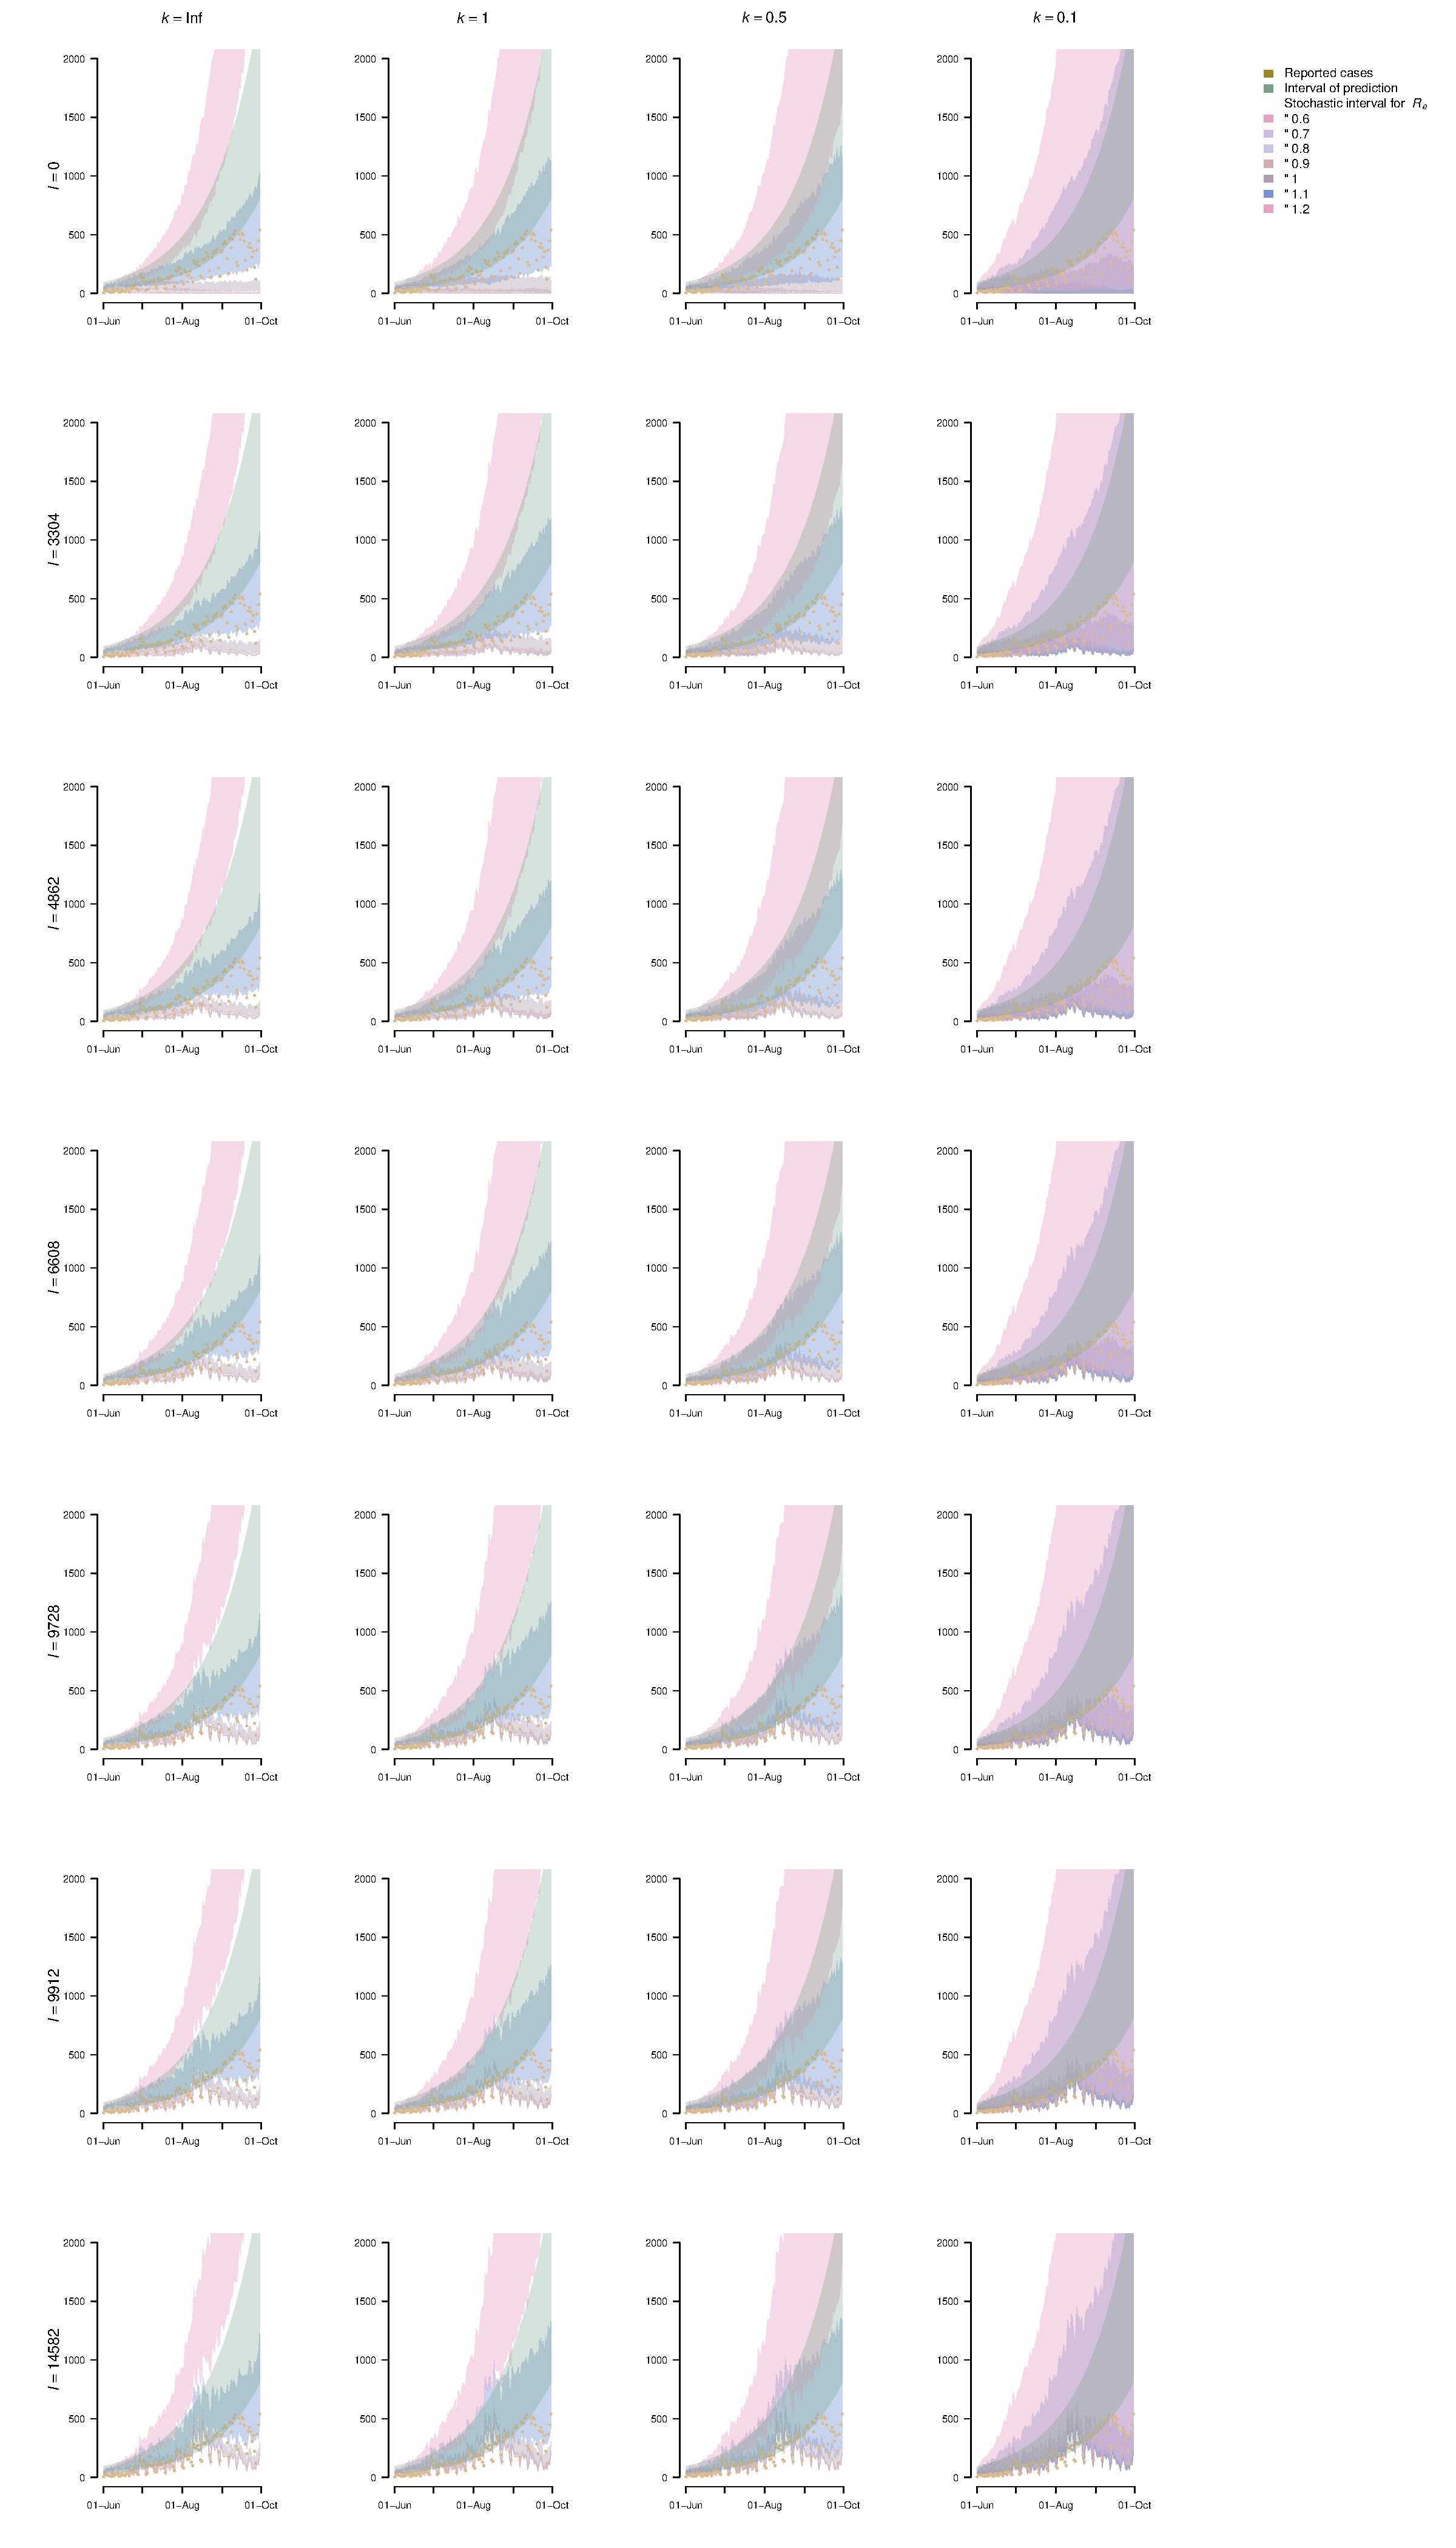
\includegraphics[scale=0.3]{sim_cases_d_imports_2021-02-24.pdf}
\caption{Impact of travel associated cases on the cases per day that do not infect further: y-axis shows the cases per day; x-axis the time of interest. Different number of travel associated cases \emph{I} were added to a stochastic branching model whereby these \emph{I} could not transmit further: \emph{I} was zero, reported \emph{I}, reported \emph{I} multiplied by $1+ \frac{\Sigma ~of ~cases ~with ~unknown ~origin }{\Sigma ~of ~all ~confirmed ~cases}$, and these multiplied with 2 and 3, respectively. Yellow dots show the reported cases per day and green area shows the predicted cases per day. Abbreviations: k, dispersion parameter; I, number of travel associated cases.}
\end{suppfigure}
\begin{suppfigure}[h]
\end{suppfigure}
\begin{suppfigure}[h]
\centering
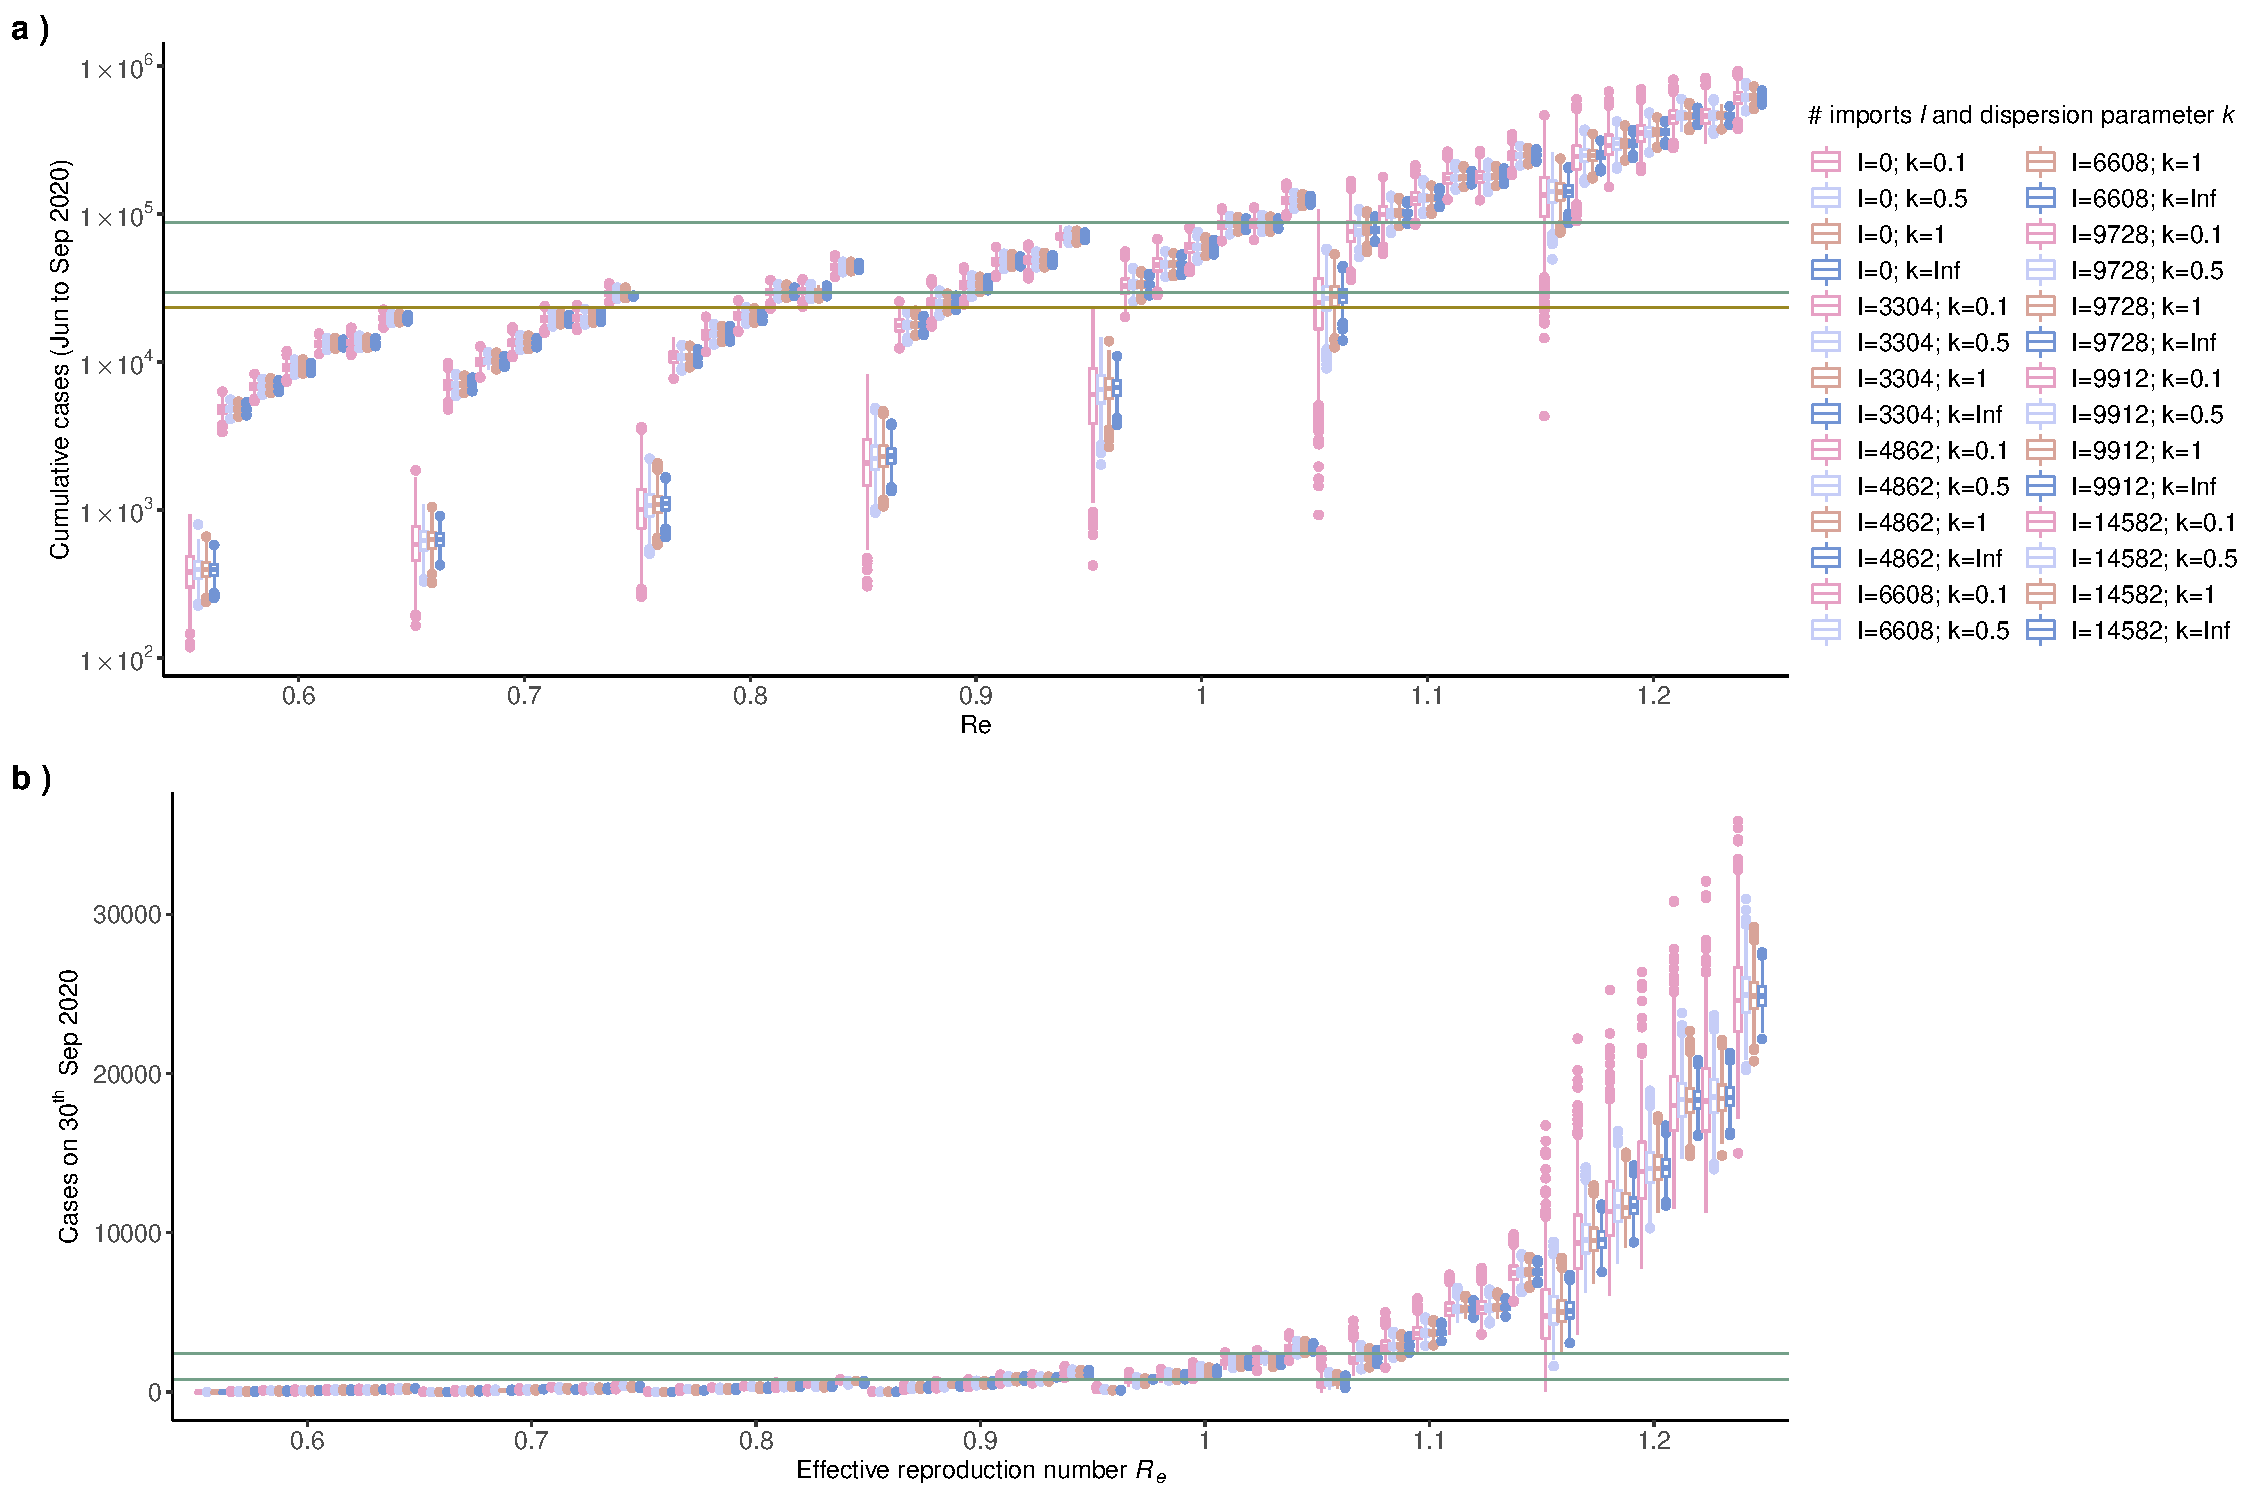
\includegraphics[scale=0.4]{size_scenarios_imports_infect_2021-02-24}
\caption{Cumulative cases and final number of cases regarding the different scenarios whereby travel associated cases infect further.Yellow line shows the reported cases during $1^{st}$ of June to $30^{th}$ of September 2020. The area between the green lines shows the predicted cases during $1^{st}$ of June to $30^{th}$ of September 2020 and on the $30^{th}$ of September 2020. Abbreviations: k, dispersion parameter; I, number of travel associated cases.}
\end{suppfigure}
\clearpage
\begin{suppfigure}[h]
\centering
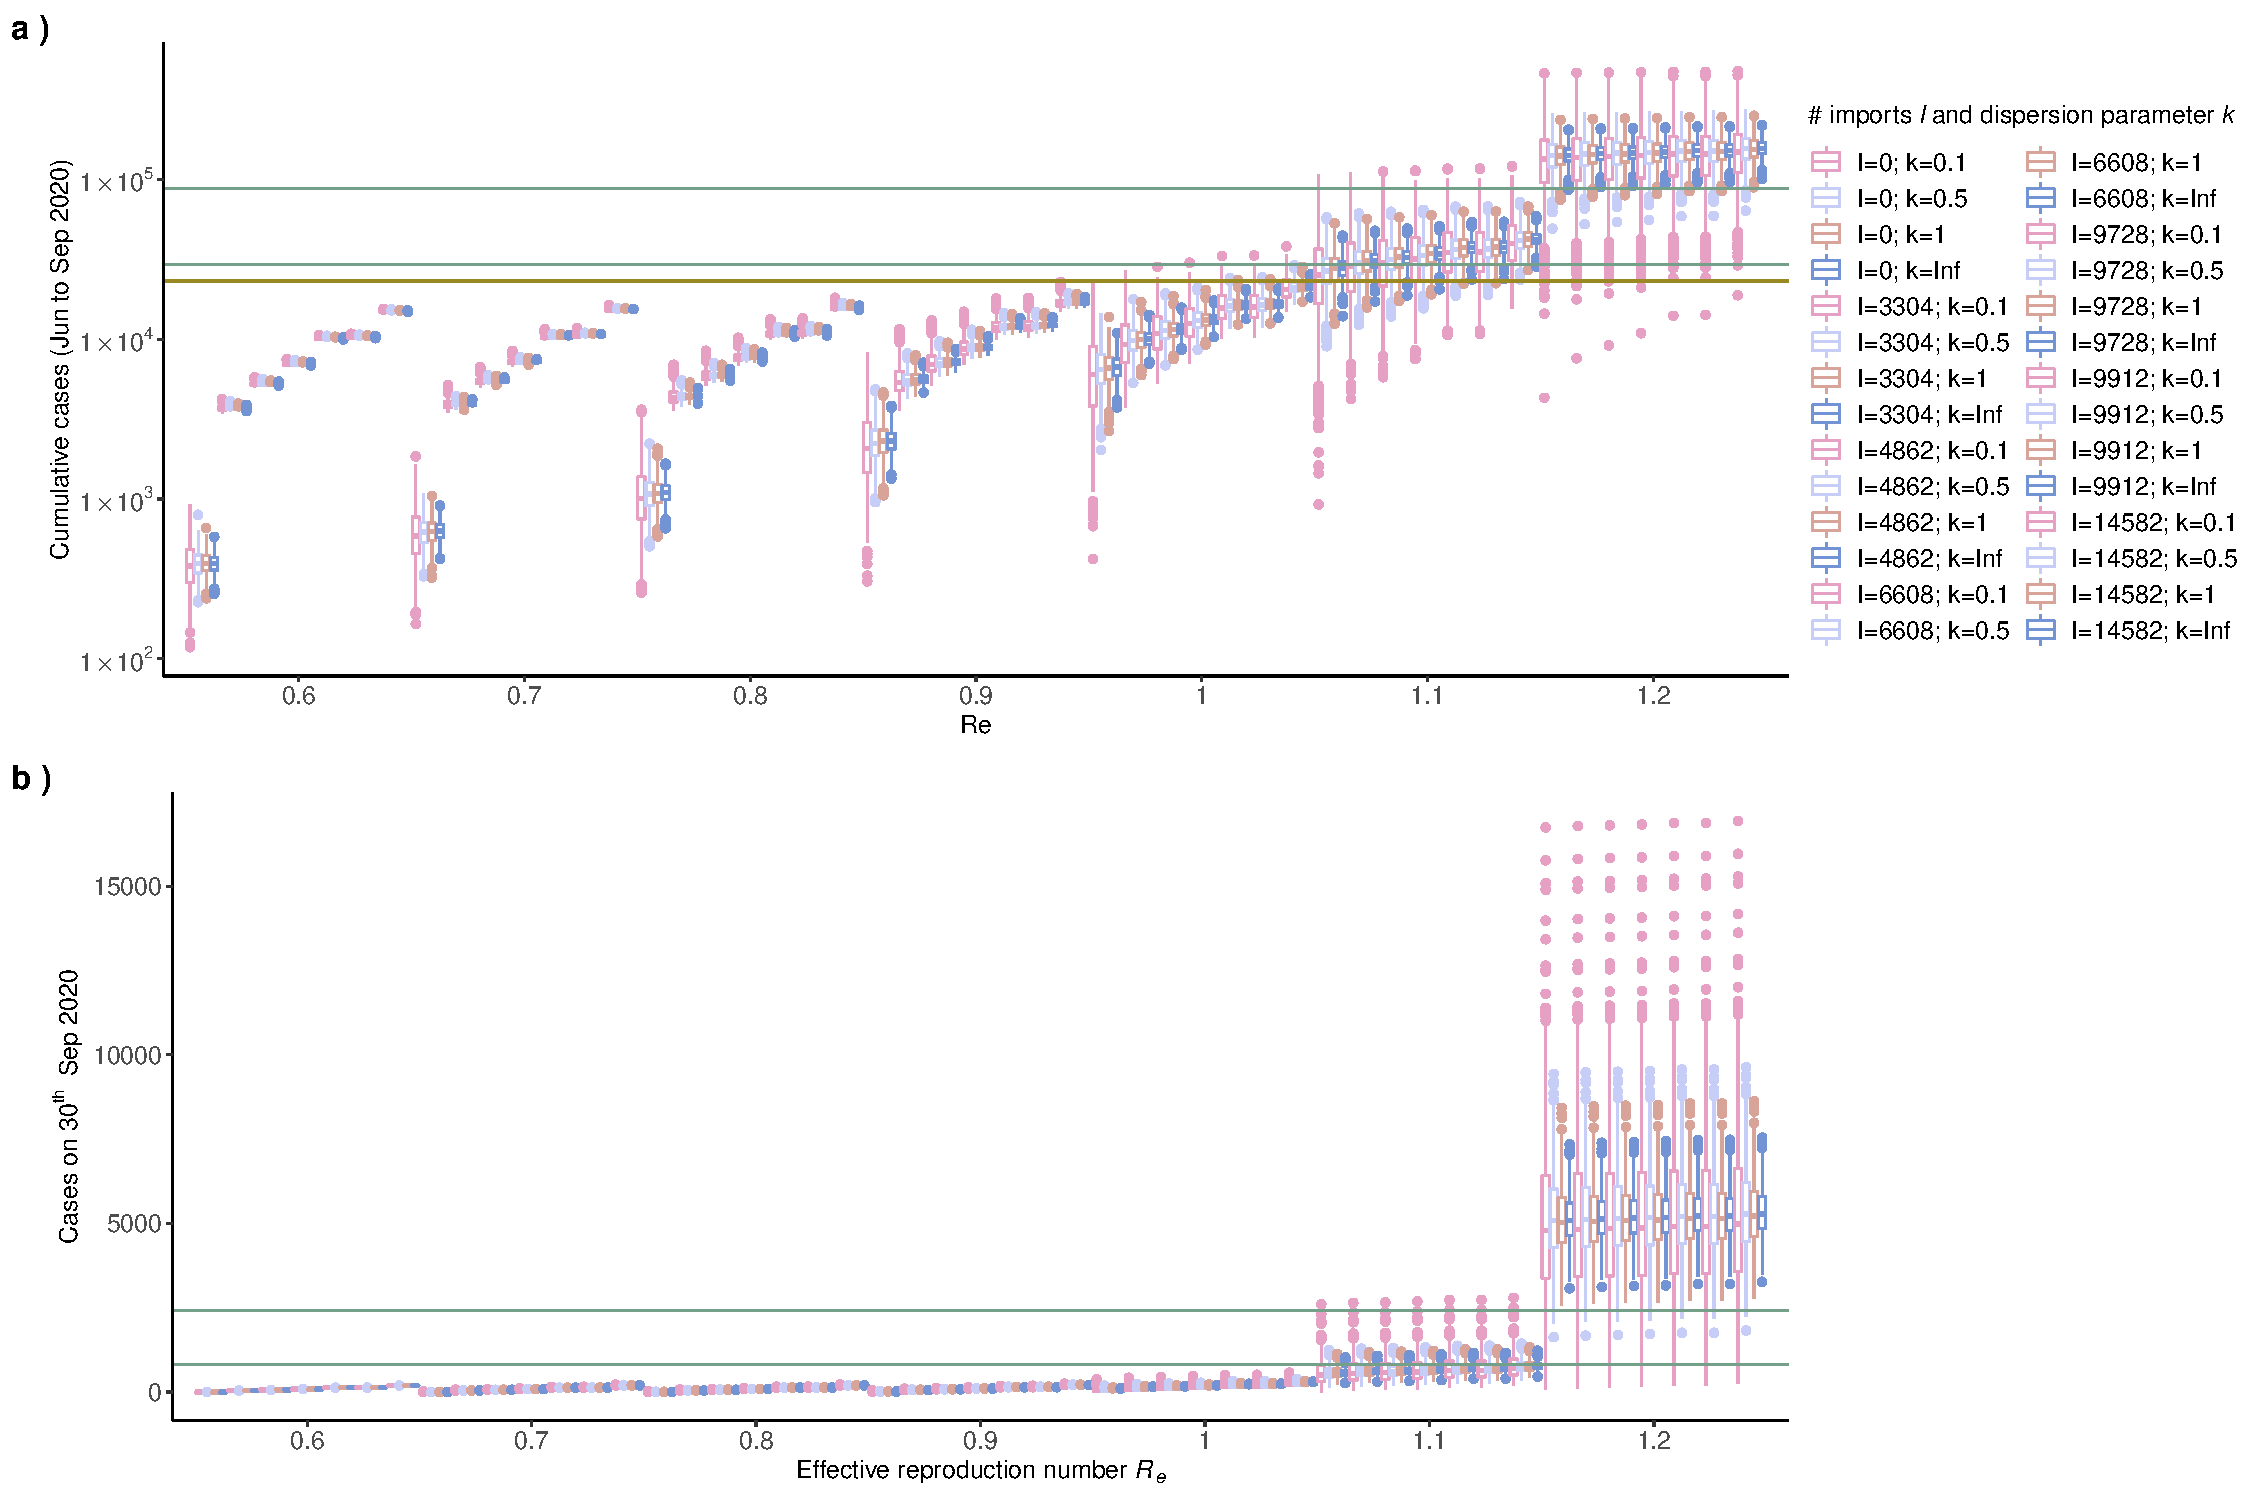
\includegraphics[scale=0.4]{size_scenarios_imports_2021-02-24}
\caption{Cumulative cases and final number of cases regarding the different scenarios whereby travel associated cases do not infect further. Yellow line shows the reported cases during $1^{st}$ of June to $30^{th}$ of September 2020. The area between the green lines shows the predicted cases during $1^{st}$ of June to $30^{th}$ of September 2020 and on the $30^{th}$ of September 2020. Abbreviations: k, dispersion parameter; I, number of travel associated cases.}
\end{suppfigure}

\end{document}




